To validate the iPad application and the features implemented, tests were carried out with various signals applied to the input pins of the Arduino and the signals were received on the app. The signals on the app could then be compared against the actual signals applied to determine how well the prototype processed and outputted the signals.



\subsection{Standard Signals}
Firstly, the prototype was tested with standard signals. The characteristic voltage applied to each input pin is summarised in Table~\ref{table: standard signals}. The A0 pin on the Arduino, corresponding to the glucose input, was connected to the ground pin on the Arduino. This was implemented to test a signal of constant voltage. The A1 pin, corresponding to lactate, was tested with a 0.1Hz square wave with a peak-to-peak voltage of 1V and a 0.5V offset. The A7 pin, corresponding to potassium, was tested with a 0.1Hz sine wave with a peak-to-peak voltage of 0.5V and 0.5V offset. 

\begin{table}[h!]
\centering
\begin{tabular}{||c c c||} 
 \hline
 Input Pin & Neurochemical & Signal Description \\ [0.5ex] 
 \hline\hline
 A0 & Glucose & Connected to Arduino GND pin \\
 A1 & Lactate & 0.1Hz square wave, 1V P-P voltage, 0.5V offset \\
 A7 & Potassium & 0.1Hz sine wave, 0.5V P-P voltage, 0.5V offset \\
 \hline
\end{tabular}
\caption{Standard signals received by input pins}
\label{table: standard signals}
\end{table}

The signals were chosen to have a low frequency since the neurochemical signals present during the occurrence of an SD display changes over a long time frame. Furthermore, the app only receives data once every second from each input, hence according the the Nyquist rate, frequencies above 0.5Hz will undergo aliasing and will not be reconstructed well. Therefore frequencies of 0.1Hz were chosen for testing.

The standard signals provided to the A1 and A7 input pins were produced by the signal generator. In parallel, these signals also went to a PicoScope input channel, which was then connected to a laptop so that the signals could be recorded on PicoLog with a sampling frequency of 5Hz. This allowed for the standard signals displayed on PicoLog to be compared with the signals received on the iPad app post processing and transmission. Figure~\ref{fig: test1} shows the set up of the experiment.

\begin{figure}[h!]
\centering
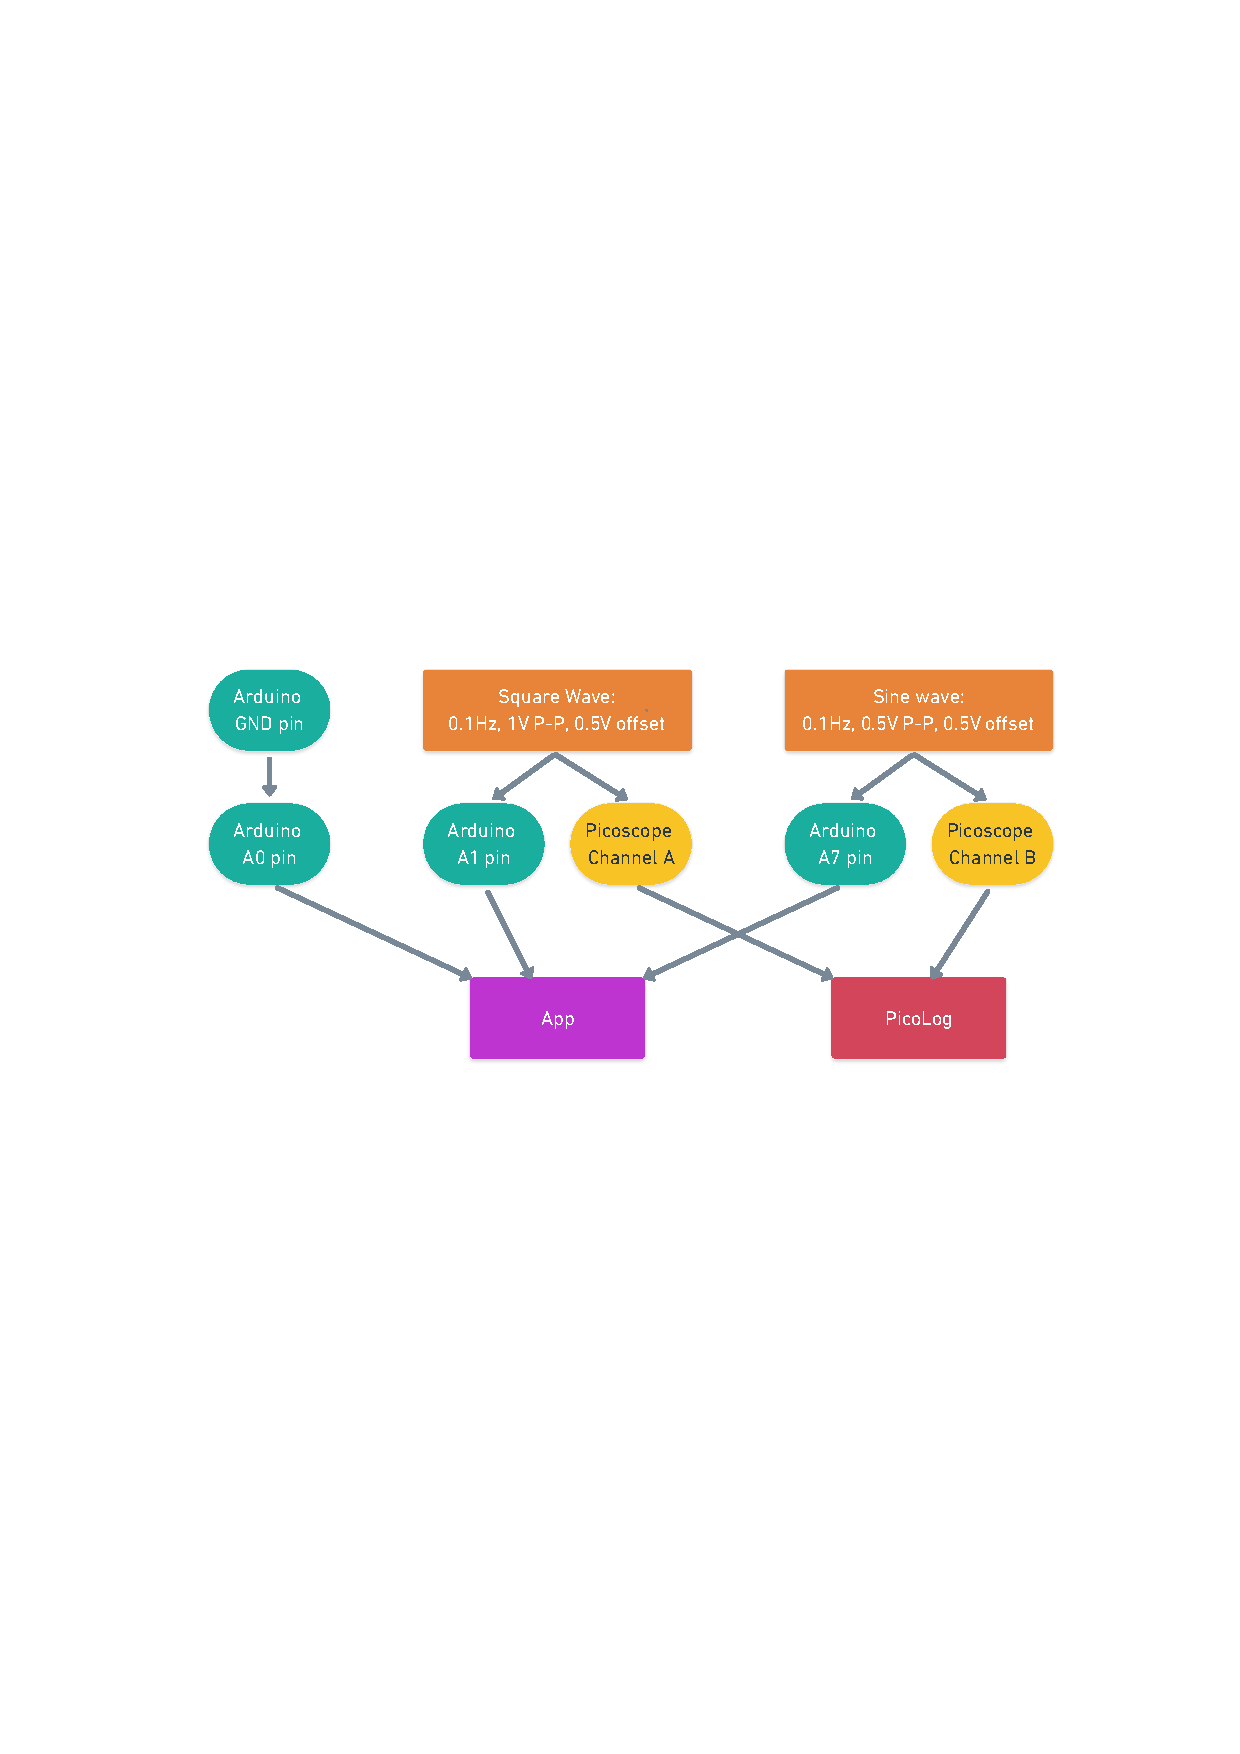
\includegraphics[trim={3cm 11cm 3cm  11cm}, clip, width=0.75\textwidth]{./figures/test1.pdf}
\captionsetup{justification=centering}
\caption{Experimental setup for testing standard signals}
\label{fig: test1}
\end{figure}

The purpose of this test was to show that the app could simultaneously receive three signals and evaluate how well the app was able to display the standard signals.

% mention limitation of picoscope so had one constant signal connected to Arduino GND pin. Fixed voltage

% purpose of the test is to show the app can receive three signals simultaneously, compare the signals with expected values on PicoLab, and show features of the app. evaluate suitability of filtering and averaging

\subsection{Brain Signals}